\chapter{A Design Space for Public Places as Infrastructure for Civic Mobile Learning}
\label{chap:DesignSpace}

Using the work covered in Chapter \ref{chap:SpacePlaceInfrastructure}---such as Star’s theories on spaces’ compositional societal infrastructures \citep{Star1999} and Dourish and Bell’s approach to the layers of meaning, practice and ritual infrastructures that constitute space \citep{Dourish2006}---this chapter explores how technologies can play a role in creating spaces where infrastructures for civic learning can be nurtured. It covers investigations held into the potential for civic technologies to support bespoke learning activities at the intersection between civic and curriculum-based learning in public spaces---in this case, public parks. It also describes the insights provided by eight months of engagements with some of the parks' stakeholders: teachers, pupils, park rangers and volunteers. These engagements included semi-structured interviews, workshops and the deployment of a prototype mobile application designed to prompt feedback and discussion. Through these engagements, we aimed to gain an understanding of the potential for mobile technologies to explore the different stakeholders' current issues and practices; explore how these can be used as resources for civic learning; and develop generalizable design requirements for future technologies for m-learning within civic space. Finally, it introduces a model of the design space for civic m-learning, and draws implications for designing platforms that support outdoor civic learning activities aimed at enhancing and developing relationships to spaces which have value to their surrounding communities. Much of the work covered by this chapter was peer-reviewed and published at Communities and Technologies 2017 \citep{Richardson2017}, with the paper being co-authored by Doctors Clara Crivellaro, Ahmed Kharrufa, Kyle Montague and Professor Patrick Olivier. 

\section{Study Context}
\label{sec:ParkContext}
As discussed in Section \ref{sec:DigitalCivics}, this project was situated within a larger socio-economic and political context of hardship currently being experienced within the UK. Significant budget cuts resulting from policies of austerity had been imposed on local government, resulting in a severe re-allocation of funds. This study concentrates on a specific consequence of this: the reduction of funding for the maintenance of local parks. Since their popularisation in the Victorian era, public parks have been a staple of British culture. Their greenery offered the working class respite from the abrasiveness of spreading urbanisation and the pollution of industry. Modern research has shown that simply having access to urban green space is essential for childhood development, as well as good mental and physical health \citep{Fiennes2015}. Today, access to green space is often limited, with 80\% of the UK’s population living in urban areas which take up only 6.8\% of its land area \citep{UKNationalEcosystemAssesment2011}. This study took place in Newcastle upon Tyne, UK, where the Newcastle City Council's Parks Service manages 12 traditional Victorian Parks, 9 countryside parks, 15 neighbourhood parks and a multitude of other sites, including several denes, reclaimed industrial sites and recreation grounds. In total, the sites managed by the Parks Service amount to over 2 million square metres of space.

Because local authorities do not have a statutory duty to fund and maintain their open spaces, local parks have had their budgets slashed under austerity measures in order to minimise the impact on other areas, such as schools and healthcare. In 2014, the Heritage Lottery Fund found that 86\% of UK park managers had seen cuts to their budgets since 2010, with some local authorities considering simply selling their parks to private investors \citep{HeritageLotteryFund2014}. Between 2010 and 2019, Newcastle City Council has had to reduce its parks budget by over 90\%. In practice, this means the loss of over 80\% of the parks' full-time staff (despite park usage increasing), increasing their reliance on volunteers from local communities.  It also means that councils are being forced to explore other ways in which parks can generate income. Many authorities have reluctantly introduced---or increased---entrance fees, and are charging schools to facilitating class trips. The combination of a loss of dedicated education staff within parks, the introduction of fees to compensate for park rangers’ time, and the schools themselves having to deal with funding issues has resulted in few schools utilising the parks as learning environments. As cost-cutting measures, even fewer take advantage of the rangers’ expertise as educational resources.

The purpose of this study is not to place greater value upon local parks than the many other elements of society which have suffered from austerity measures. Instead, it serves as a case study exploring how issues which affect places as outwardly simple as parks can impact a large number of community stakeholders in many different ways, and how mobile technologies might use that as a platform for learning and sharing those stakeholders' values.

\section{Identifying the Research Domain: Parks2026}
\label{sec:Parks2026}

\begin{figure*}
  \centering
  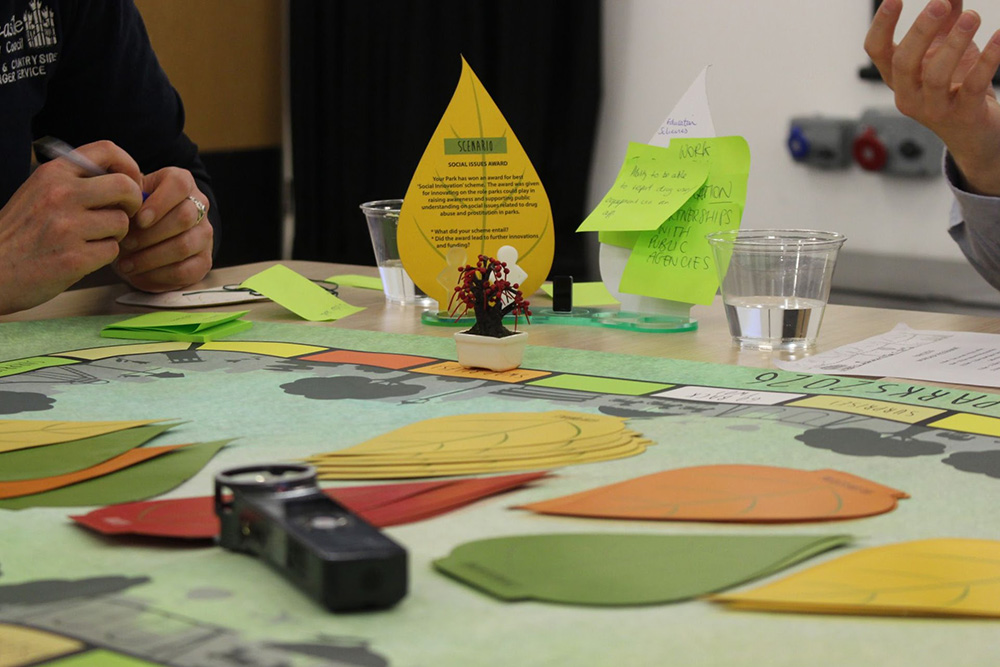
\includegraphics[width=0.8\columnwidth]{images/chapter04/parks2026.jpg}
  \caption{Participants engaging in the Parks2026 workshop board game.}
  \label{fig:parks2026}
\end{figure*}

A larger Open Lab project had started in 2015, with the aim of researching the potential for digital technologies to mitigate the impact of austerity politics on Newcastle's parks services \citep{Crivellaro2019}. I joined the project's initial engagement process, dubbed `Parks2026', in an effort to find a context to engage with for my PhD. The Parks2026 process consisted of an exploratory workshop, which investigated the value of local parks as a general community resource and offered the various stakeholders opportunities for opening dialogue around the future of the parks. As well as the general value and use cases of parks as community resources, the workshop aimed to act as a scoping mechanism: investigating the current practices and attitudes towards technology held by park staff, volunteers and council representatives. The workshop was attended by 25 participants (mostly staff and volunteers, participants noted the absence of several invited council representatives). Discussion was aided through the introduction of a group board game, which asked its players to envisage their park ten years in the future (Figure \ref{fig:parks2026}). Participants played the game in groups of 4-5, with discussions being audio-recorded and decisions noted down by an elected group member.

The game utilised provocative `scenario cards' to probe the players’ thoughts on specific hypothetical near-future scenarios, based upon earlier discussions with the project's prior participants. The scenarios were grouped under the categories of community engagement, governance, volunteering, maintenance and values. These addressed issues such as the players’ favourite aspects of their park, the democratisation of it as a resource and the introduction of technology in the organisation of volunteers. Amongst these topics were also several related to event organisation, the collection of volunteers’ experiences, park-based community curriculum and situated learning mobile applications. Participant groups were asked to discuss the scenarios, and agree on potential solutions or approaches in response to them.

It was immediately obvious that the participants cared deeply about the parks, and saw them as a resource integral to the surrounding community. However, it was also clear that the parks held value in multiple areas. The subject of health (both physical and psychological) and well-being was brought up repeatedly, and they were also noted as being an environment well suited to socialising. This seemed particularly true for groups such as the elderly, who might not have many other socialising opportunities.

However, one aspect which many of the park rangers and volunteers seemed particularly eager to emphasize was the role of the park as an educational resource. They saw school trips and other similar activities as an opportunity to not only increase the park’s perceived value to the community through its use, but also to expose and encourage a new generation to become future ‘wardens’:

\begin{displayquote}
"Well it does give you the opportunity to engage on a more long-term basis with different groups---say a youth group to like the art, or schools or something like that. To develop some relationship."
\end{displayquote}

\begin{displayquote}
"Well the potential benefit is enormous, because it means that a group of people will hopefully become involved in the park in a continuing fashion."
\end{displayquote}

Participants were also keen to point out that the benefits of this relationship flowed both ways, and that schools had much to gain from the park as a physical resource and the expertise of the park rangers. They describe something alike to parks evolving a symbiotic relationship with nearby schools:

\begin{displayquote}
"Well, I suppose that's why you have to have the park staff working with teachers: the park staff know the park, and the teaching staff know what works as good education."
\end{displayquote}

From these discussions, it became clear that the individuals involved with the parks---both employees and volunteers alike---saw a huge amount of value in them as educational resources, but were simultaneously frustrated that they were going underutilized by the surrounding schools. It was these findings that first got me interested in researching the intersection of community space, technology and education. I decided to further investigate how the parks were being used by schools and the potential value of parks as learning resources.

\section{Exploratory Field Studies}
Several visits to multiple parks were held to understand the learning resources that they offered, how they were being used by schools, the attitudes towards the parks by their local communities and the time and budgetary constraints that the park rangers had to deal with. Five parks were visited, varying from one of the more deprived areas of Newcastle to some of the most affluent. Unstructured interviews were held with the rangers at each site, typically as we toured the grounds.

There was a positive correlation between an area’s prosperity and the amount of community support given to its local park. For example, Gosforth Central Park was widely known amongst the rangers for the number of its community volunteers: roughly 20 volunteers perform maintenance work in the park on a weekly basis, with several times that number volunteering in some less regular form. The volunteer group `Friends of Gosforth Central Park' (\textit{`Friends of X Park'} is a common naming convention for park volunteer groups) also had an active presence on social media. The surrounding area is fairly affluent, and has being named as one of the best places to live in Britain \citep{TheSundayTimes2015}. In comparison, despite being larger, Walker Park---based in one of Newcastle’s more deprived areas---saw only five or so weekly volunteers. 

Attitudes towards the use of the park by young people also varied according to area: for example, according to the ranger of Walker Park, some of the local community have been resistant to her efforts to introduce extra-curricular outlets for young people in the area due to fears of vandalism. Secondary schools had also almost entirely stopped visiting the park---something she was extremely keen to rectify. In comparison, Gosforth Central Park has been actively coordinating with local schools on several projects, including the design of a new pond space. The leading volunteer of the park claimed that they hoped to get the children invested in the park from an early age, so that they could contribute towards its maintenance later in life or at least appreciate and respect the park as a community space. 

Despite all of the visited park rangers confirming that schools’ usage of the park had significantly decreased in recent years, some school trips were still occurring. A school trip to Walker Park was observed, where a large class of young children (N=36, age=5-6) were taken by the park ranger on a hunt for minibeasts. This was linked into the class' current book at school, \textit{The Hungry Hungry Caterpillar}. The park ranger was the sole content deliverer for the session, despite multiple teachers being present (necessary for large groups) and her lack of teaching experience. The teachers deferred to her expertise on the given subject and relegated themselves to `crowd-control'. The class clearly enjoyed the lesson, being particularly excited about being in the park environment and going hands-on with the bug hunt. The ranger supplied the group with simple equipment and tools---such as specimen jars and magnifying sheets---which the children relished in using and were reluctant to share between themselves. The children held an obvious desire to share their findings with anyone and everyone around them, particularly relishing the attention of the adults of the group. These discoveries, such as snails and worms, were photographed by the adults through the use of several iPads. The teachers claimed that the photos were to be put on display on return to the classroom, and the devices never left the adults' hands.

\begin{figure*}
  \centering
  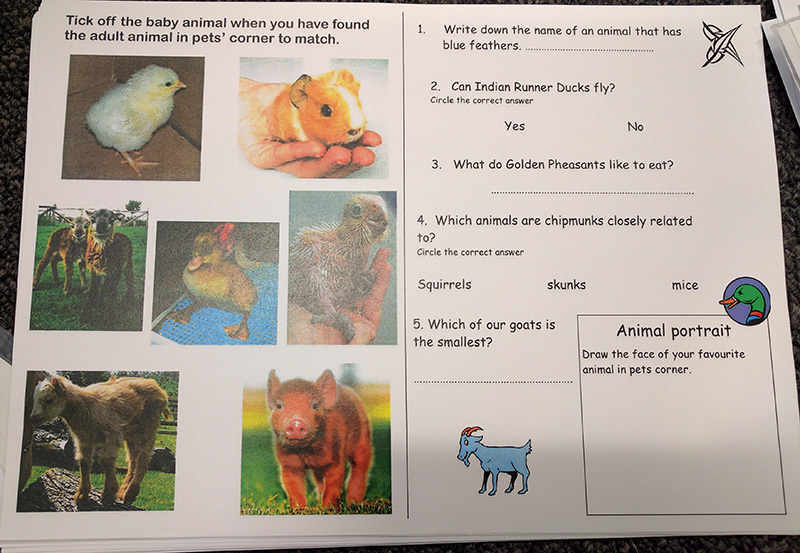
\includegraphics[width=0.8\columnwidth]{images/chapter04/worksheet.jpg}
  \caption[An existing park worksheet]{An example school worksheet, created by the Jesmond Dene educational officer.}
  \label{fig:worksheet}
\end{figure*}

A visit to Jesmond Dene park showed that it had also been struck severely by the budget cuts. It features an educational petting zoo called \textit{`Pets' Corner'} (which introduces young children to farmyard animals and exotic birds) and a wildlife reserve area complete with a pond, bird feeders and houses as well as wild grass and flowers. The park also boasts an sizeable and modern indoor facility dedicated to educational activities (featuring desks, chairs, projector and smartboard) and a large number of educational resources such as worksheets and pre-made activities (Figure \ref{fig:worksheet}). However, the reduced budget has meant that there is no longer a dedicated educational officer in the park. Without an educational officer no new educational activities have been produced and school trips have to be facilitated by the park ranger. Having not made them, the ranger was understandably largely unfamiliar with the learning resources and activities. Furthermore, she also had to charge schools for her time, as she still had other responsibilities. The learning resources themselves were relatively simple, with the majority of them taking the form of paper worksheets. Due to the younger nature of the target audience, most of them prominently featured images and simple text instructions with very few of them requiring the children to write significant amounts of text. Nearly all of the worksheets relied on the children being physically present in the park in order to answer questions about the plants and animals found within it.

\begin{figure*}
  \centering
  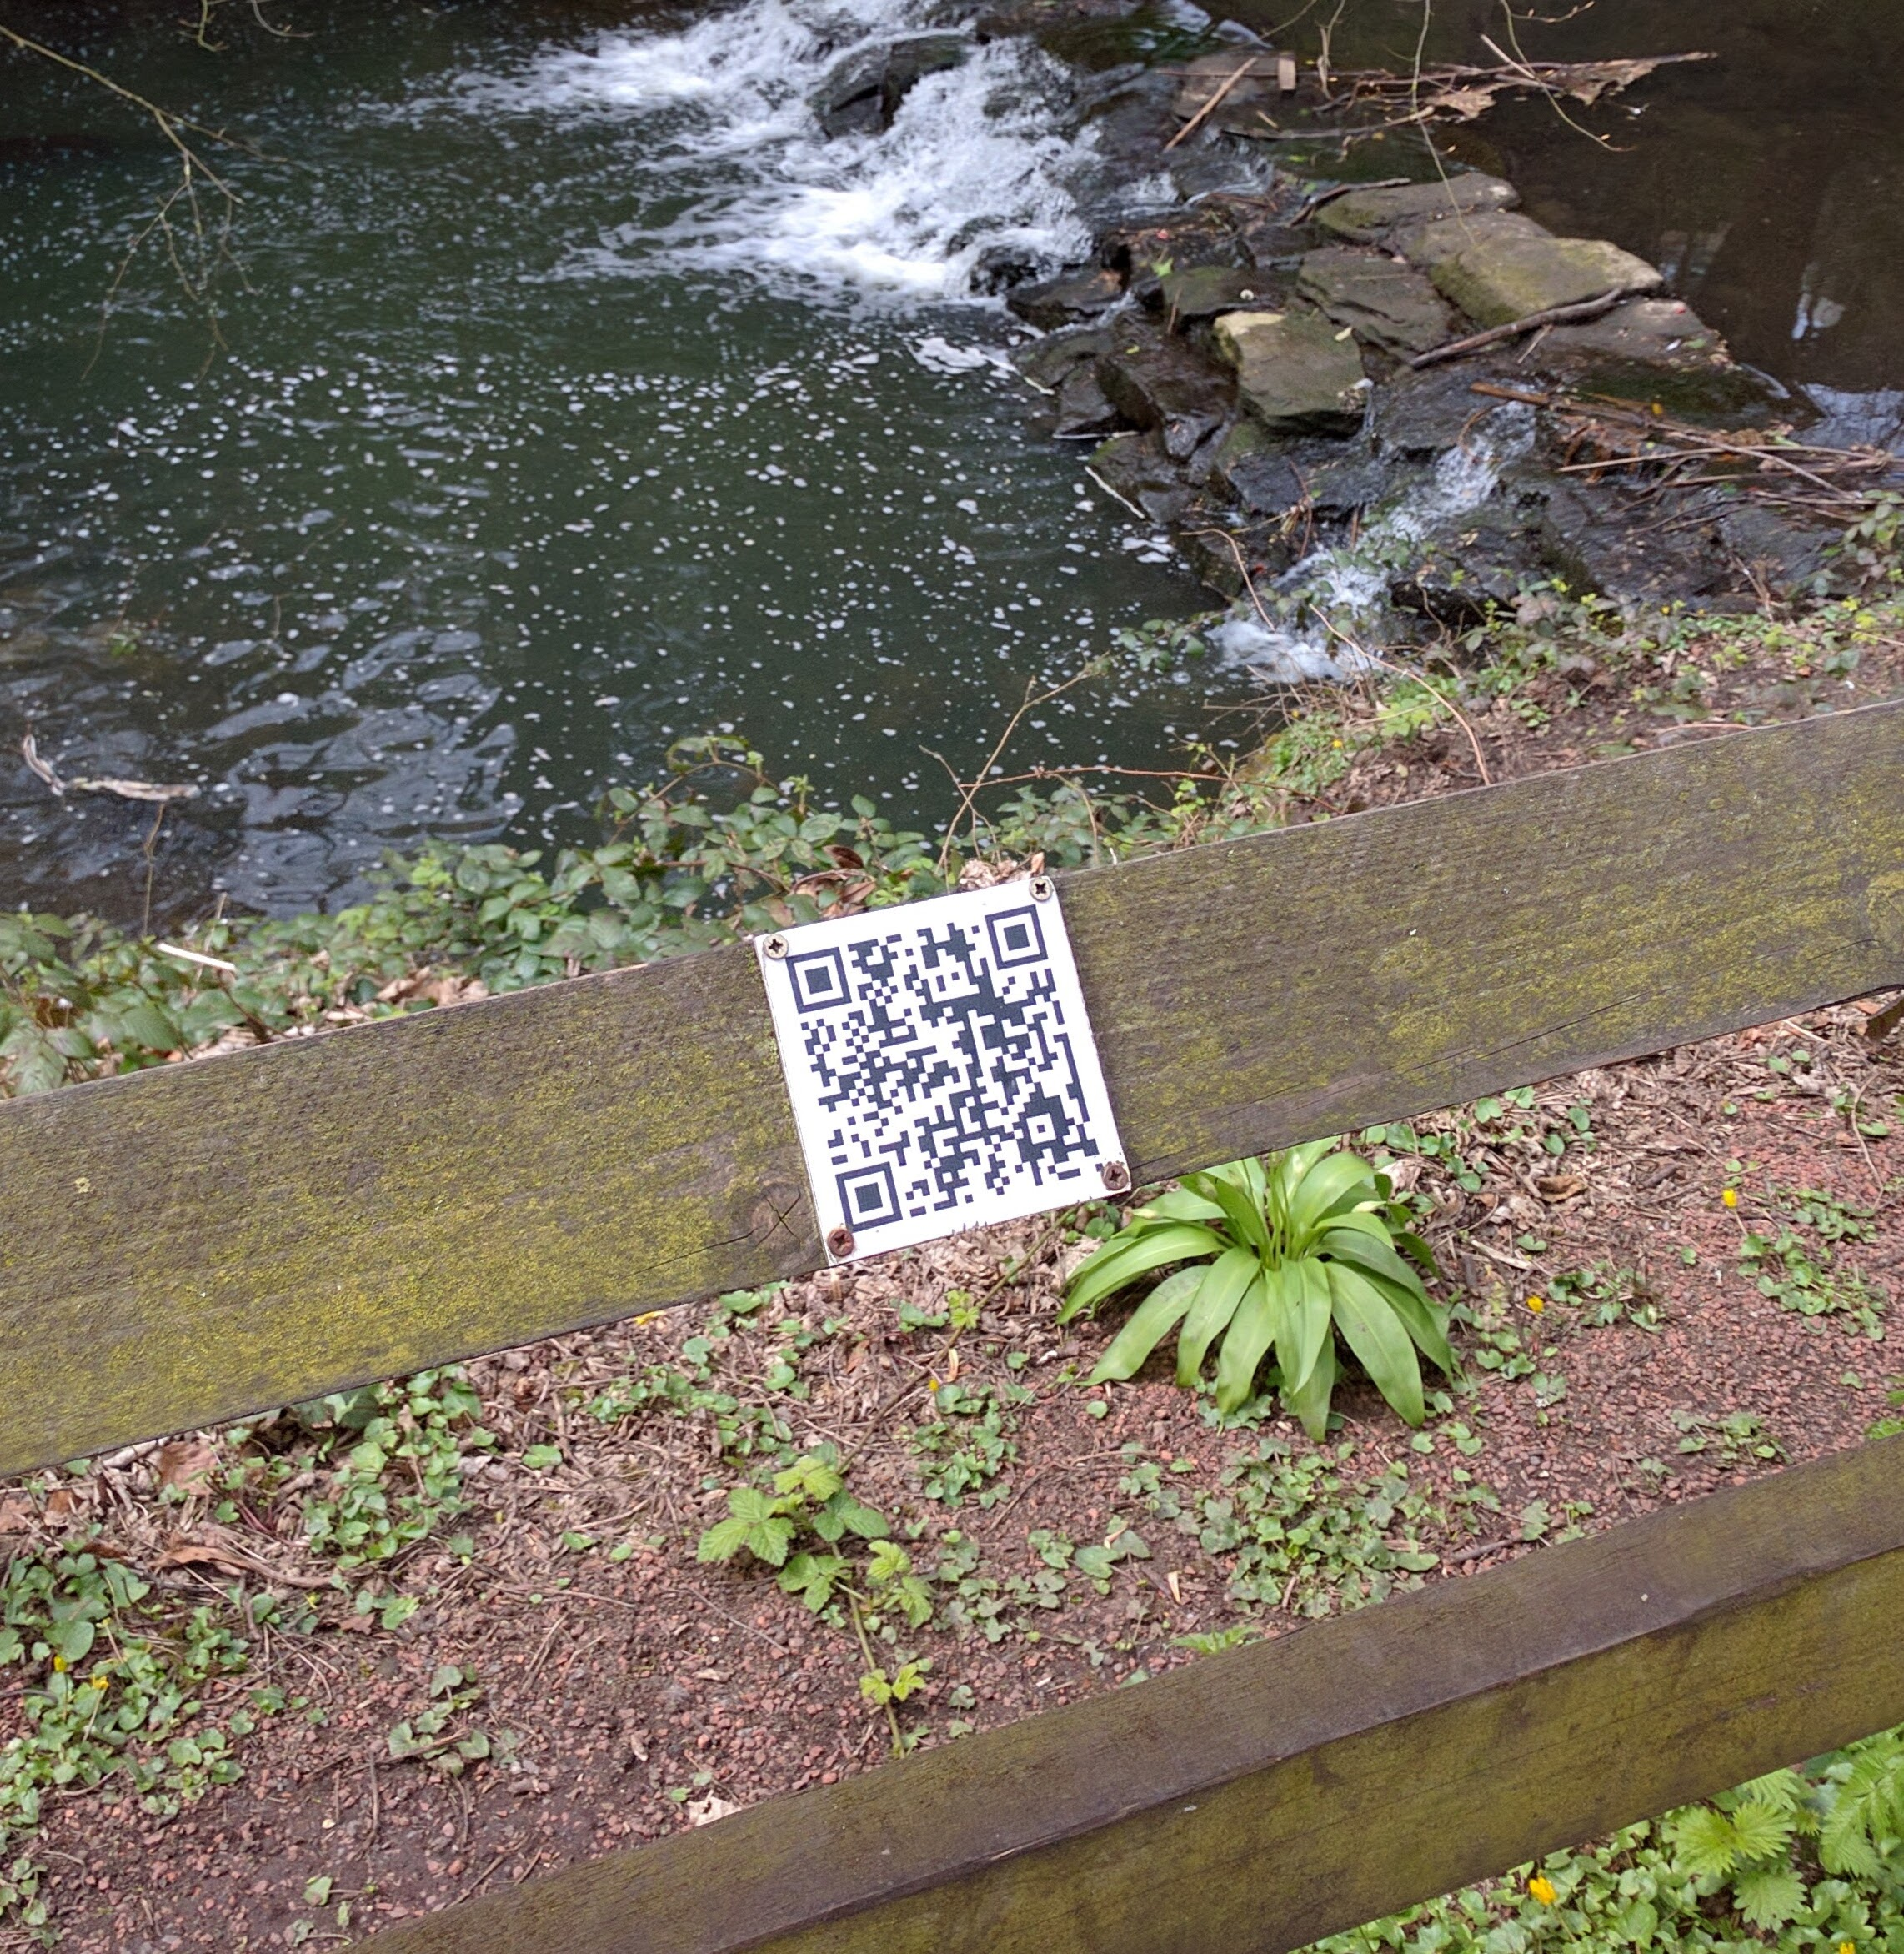
\includegraphics[width=0.6\columnwidth]{images/chapter04/jesmondQR.jpg}
  \caption[An existing QR code in Jesmond Dene]{A QR code found in Jesmond Dene, linking to a wildlife information website.}
  \label{fig:jesmondQR}
\end{figure*}

Jesmond Dene had also already utilised technology for educational purposes in multiple ways. QR codes distributed around the park which linked to wildlife information websites when scanned (Figure \ref{fig:jesmondQR}). However, these QR codes lacked any context prior to being scanned, such as what they data they contained, what subject in the park they were related to, who installed them and how to actually scan them. Even the rangers didn't seem to know much. The rangers claimed that few people seemed to interact with the QR codes, potentially because of this ambiguity. The visitor centre featured both a tabletop display and a digital kiosk. The tabletop interface displayed a custom website, featuring a map of the park; an overview of the park's history, comparing historical photos with modern ones; historic points of interest; and an interactive quiz regarding features, plants and animals of the park. The kiosk boasted a touchscreen and speakers, and allowed for user generated content such as images and video of the park to be publicly displayed. However, the rangers noted that neither of these pieces of equipment were frequently used, and that the table top interface was prone to frequent crashing.

\section{Initial Application Concept}

From these observations and findings, we came to believe that the rangers and schools would benefit from a mobile application which simplified the processes of creating, organising, sharing and consuming park learning materials. In order to take advantage of each park’s unique assets, the application would have to allow for rangers and teachers to easily design learning activities on a per-park basis. These activities would be delivered to the children through the same application in an outdoor, mobile learning context. The initial findings from these early engagements suggested that even young children would be very comfortable using mobile technologies, and that they would better engage in activities which allowed them elements of independence and creative control. 

Following a review of the literature as covered in chapter \ref{chap:MobileLearning}, we had a clearer picture of an initial application design. It should allow for the creation and sharing of activities designed for situated learning, utilising the park as a physical context. Experts from the local community should be able to contribute their knowledge, experience and outlooks through the creation of these activities, allowing learners to also engage with the parks as \textit{places}. However, we noted that care must be taken to avoid simple content delivery for the learner, allowing them some degree of creative control to boost engagement. The learning activities should also be designed for use by small groups or pairs, encouraging communication, teamwork and social skills.

Based on these established requirements for such a system, we designed a model by which existing learning activities could be adapted into a modular format, suitable for later translation into a digital application. We used worksheets we had found in the parks into activity topics, then broke them into smaller tasks which required a user interaction. For example, a worksheet could hold the activity topic of "Animals in Pets' Corner" and include tasks such as drawing and multiple choice answers. As the medium of mobile technology afforded more complex interactions than a simple pen and paper, I also noted several additional interactions could make use of current mobile technology, such as photography, audio recording and GPS map-marking.

\section{Park Staff \& Teacher Paper Prototype Workshop}
\label{sec:PrototypeWorkshop}

We held a workshop to understand the impacts of this context on the parks’ various educational stakeholders. This workshop was attended by a combination of park rangers, volunteers and teachers. We wanted to explore the participants’ thoughts on the initial design concept and, if supported, co-design its potential features and learning activities.

\begin{figure*}
  \centering
  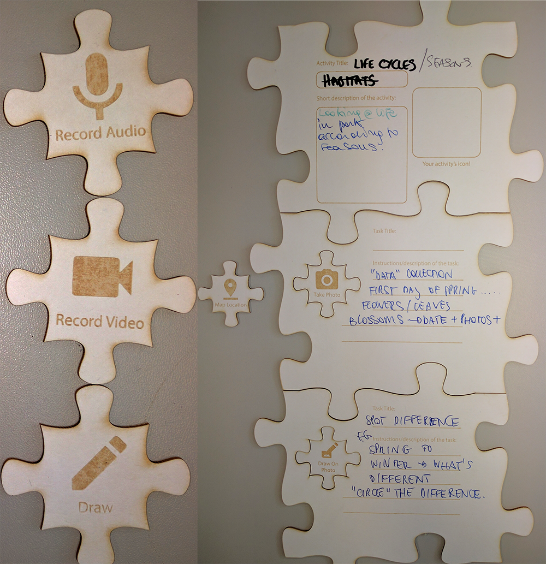
\includegraphics[width=0.8\columnwidth]{images/chapter04/rangerJigsaw.png}
  \caption[The jigsaw prototyping activity]{The paper prototype jigsaw workshop activity, used with the rangers and teachers to ideate m-learning activities and prompt discussion around the initial application concept.}
  \label{fig:rangerJigsaw}
\end{figure*}

In order to make the modular relationship between these tasks and the larger activities more clear, we conceived a paper prototype in the form of physical laser-cut jigsaw (Figure \ref{fig:rangerJigsaw}). Each jigsaw consisted of a root piece which could be filled in to detail the activity’s subject, and multiple other pieces which represented the tasks that the learner would be asked to complete. The pieces were designed to be as configurable as possible, allowing for simple, non-linear or even cyclic activity design. The user interactions were represented by their own, smaller pieces. Some of these were left blank, to allow for participants to suggest ideas for the types of interactions the application could have. Others consisted of the interactions noted earlier which utilised the mobile technology (e.g. recording video), or ones which conformed to the existing learning materials (e.g. drawing a picture). The jigsaw activity was designed to be highly tactile (encouraging the participants’ curiosity and for them to experiment with re-configuring the activities they created) and visual (allowing participants to work in small groups and communicate ideas easily).

Using the jigsaw activity, the participants identified a number of potential themes for mobile learning material, including habitats, life cycles, maths, growing food, history, physics, citizenship and healthy living. Overall, they were positive about the idea of creating and sharing digitised mobile learning materials. However, several concerns were voiced which the a final system design would need to take into account. The teachers noted that for a system such as this to be used by schools, it would likely have to be able to show a proof of each child’s learning, understanding and their progression over time. There was also a concern that if these activities were to be created by anyone in the surrounding community, they would have to be screened and vetted for appropriateness before being made visible to children.

However, the participants struggled to understand the jigsaw metaphor and didn't meaningfully engage with the paper prototype. We suspected that the jigsaw was too abstract for the participants to clearly understand without first seeing a working version of the app: its modular structure was complicated enough that a more functional prototype was likely necessary to clearly demonstrate both our intentions and the application’s potential. The teachers were also verbally reluctant to write on the pieces, seeing them as reusable learning resources which shouldn't be written on.

\section{Application Prototype}

\begin{figure*}
  \centering
  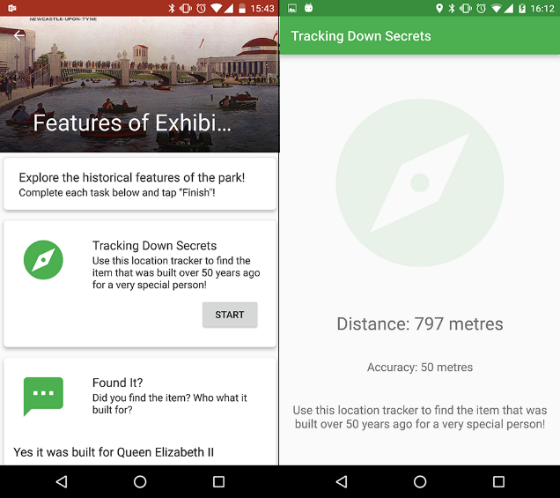
\includegraphics[width=0.8\columnwidth]{images/chapter04/parklearnprototype.png}
  \caption{The prototype Park:Learn application.}
  \label{fig:parklearnPrototype}
\end{figure*}

While the participants had been receptive to the idea of a mobile learning application for park educational activities, it was clear that the jigsaw was too abstract of a prototype to gain much useful feedback. We also realised that to gain an understanding of children’s attitudes towards the parks and technology, something more appealing would be necessary to engage them. The initial findings from these early engagements suggested that even young children would be very comfortable using mobile technologies, and that they would better engage in activities which allowed them elements of independence and creative control. From these findings---and insights gained from studying prior work---a mobile learning application prototype was developed for use with children on school trips, as well as adults in further workshops. This allowed us to gain insights from participants in a more fun, interactive manner than the previous engagements.

Park:Learn (the prototype Android application) acted as a technology probe, offering a number of modular interactions which could be configured together into outdoor learning activities (Figure \ref{fig:parklearnPrototype}: left). The application was developed for Android mobile devices using Xamarin, a mobile development platform which utilises cross-platform implementations of the .NET framework to allow for a largely shared codebase between Android, iOS and the Universal Windows Platform \citep{Xamarin2016}. Android was selected for this prototype, due to its abundance and the ability to rapidly deploy onto the Google Play platform. However, the use of Xamarin allowed for future versions of the application to share a codebase between multiple mobile platforms. More detail about the application's development and implementation can be found in chapter \ref{chap:Design}.

This prototype version featured a number of learner interaction types, including taking a photo (`\textit{Take a Photo}'), matching an existing photo using a translucent image overlay on the camera (`\textit{Photo Match}') recording video (`\textit{Record Video}'), recording audio (`\textit{Record Audio}'), drawing digital pictures (`\textit{Draw a Picture}'), drawing on top of taken photos (`\textit{Draw on Photo}'), marking a location on a Google Maps view (`\textit{Map Marking}'), tracking down a location by the device’s distance from a geo-coordinate (`\textit{Location Hunt}', Figure \ref{fig:parklearnPrototype}: right), choosing between pre-written answers on radio buttons (`\textit{Multiple Choice}') and simple text entry in an empty textbox (`\textit{Text Entry}'). Each of these interactions were chosen either because they put an element of creative control into the hands of the learner, took advantage of the devices’ hardware capabilities or—as in the case of Multiple Choice and Text Entry—emulated features of the learning materials currently in use. Unlike projects such as Ambient Wood \citep{Rogers2004} and Explore! \citep{Costabile2008} (which required additional equipment or the production of 3D graphics), Park:Learn activities can be self-contained within the device and very quick to create due to the app’s modular nature. In the task model for mobile learning \citep{Sharples2013}, these features allow activities to be designed which are intrinsically linked to the context of the park, use a wide variety of tools which allow for content construction, offer the learner a large degree of control and (for the group activities) cooperation and communication. 

Unlike later versions, the prototype did not allow for the creation of new activities within the app itself. Nor could they be loaded from from a remote server, as this had not yet been developed. Instead, activities had to be manually written in the JSON (JavaScript Object Notation) data format and hard-coded into the app. I created some sample hard-coded activities prior to the following engagements in order to demonstrate the application's functionality. These activities were based on the existing worksheets and activities witnessed during the previous site visits.

\section{Prototype Engagements}

With the functional prototype in a usable state, we held further engagements with the various park stakeholders to further understand the potential roles for mobile learning technologies within civic spaces. These engagements consisted of workshops with adults (one with teachers, another with park rangers) and a deployment of the prototype with children attending a local summer school near a large park. The workshops were made up of short activities and semi-structured group discussions focusing on the participants’ relationships with parks as places, their use of the parks as learning environments, their general experiences with outdoor learning, their use of educational technologies and their thoughts on this design concept.

This section will give an overview of these individual engagements, with section \ref{sec:InfrastructureInsights} detailing the themes which resulted from a qualitative analysis across all of them combined. The methods used for data collection and thematic analysis conformed to the approach detailed in section \ref{sec:ResearchApproach}. 

\subsection{Teacher Workshop}

We organised another workshop with teachers of various disciplines (N=5). As it took place during the UK's summer school holiday period, these teachers were hired for the afternoon through a supply teacher agency. The goal of this workshop was to discuss the teachers' previous experiences with outdoor learning, as well as their ideas for what activities and interactions could be created for the application. The teachers appeared genuinely excited following a short live demo of the application. In contrast to the previous workshop, the participants seemed to understand the concept and saw potential in the idea.

The majority of the teachers had substantial experience with teaching outside the classroom, and all reported that they would like to more regularly incorporate outdoor learning into their teaching. They also noted that the introduction of the national curriculum had affected the flexibility of teachers of older students (particularly Key Stage 3 and above), meaning that fewer trips tended to take place. 

They claimed that there was a multitude of obstacles that stood in the way of a teacher being able to hold an outdoor lesson. The most obvious of which was cost, with transport being the biggest expense. However, other issues such as the bureaucracy related to health and safety and short lesson times were also mentioned. One of the more interesting issues was related to the negative social perception of learning outside of the classroom: they noted than many parents see it as "slacking off". One physics teacher explained how he had received a complaint from a parent who had glimpsed him teaching on the school field, despite the lesson being very successful. He posited that a good counter to this was being able to provide evidence of learning, proving that the lesson had been fruitful. The teachers noted that this had to be taken into account when planning each course’s `scheme of work'---a pre-prepared teaching plan which maps out how resources, activities and assessment strategies will be used in order to meet particular learning aims and objectives. The teachers were adamant that the children’s tech-literacy wouldn’t be an issue from Key Stage 2 and above. One teacher recalled that she had even taught a class of 7 year-olds that ran their own blogs.

In response to the abilities of the application, the teachers created a large number of topics and activities well suited to mobile learning technology in parks. These included conventional school subjects such as biology, art, design, textiles, geography and physics, however there were also ideas related to preparation for the Duke of Edinburgh’s Award (a youth programme featuring self-improvement exercises). Some of the imagined user interactions included map reading and writing, path-finding, video recording and analysis, triangulation, measuring parallax through photography and recording environmental audio.

With the background research having shown that children engage more with work when their creative output is put to use \citep{TheNationalEnvironmentalEducationFoundation}, we were particularly interested in how the teachers might use any materials that children generated through the app (such as drawings, photos or map data) in future lessons on return to the classroom. Multiple ideas were floated, including the creation of multimedia collages using the collected photographs, audio and video, designing textiles by using photographs as source material and peer assessment.

\subsection{Park Ranger Workshop}

With a greater understanding of the teachers’ perspective, we organised another workshop with the park rangers (N=3) exclusively, aiming to game some further insight into the specifics of educational practice within the parks. The rangers clearly had a lot of practise hosting educational events and activities in the parks, with some participants boasting several decades of experience.

The subjects that the rangers reported to have taught in the park was extremely diverse. While the most common topics usually were related to biology (often focusing on habitats and invertebrates), they had also taught children subjects such as the social history of the surrounding area, geographic topics such as erosion and river tributaries and the impact of humans of the environment. As in Jesmond Dene, a very large collection of educational worksheets had been amassed. However, the poor organisational structure meant that if a particular activity was required it would have been difficult to re-acquire.

The rangers all agreed that the introduction of the National Curriculum had a large impact on how the park was used for education: while previously many of the educational activities had taken a holistic, free-form approach to the general appreciation and protection of nature, teachers now had to ask for very specific topics to be covered in order to fit into their curriculum plan. The national curriculum also affected the demographics of the park’s educational activities: due to the more focused structure and requirements of the later stages of education, the number of visits by Key Stage 3 (11-14 years old) groups dwindled. According to the rangers, the current most frequently visiting age group is Key Stage 1 (5-7 years), followed by Key Stage 2 (7-11). This was in line with the teachers’ experiences.

Another talking point was the funding cuts to both parks and schools. Once the funding to the parks started being cut, they had to start charging schools for trips in an attempt to compensate. Unsurprisingly, the rangers claimed that as soon as the charges to schools were introduced the number of visits from them "dropped off".

The discussions also revealed that the rangers were largely unhappy with how the disruptions caused by the lack of funding had affected their day-to-day jobs. The lack of resources available to them meant that they had to shoulder more physical work related to their park’s upkeep (such as litter-picking) and had less time to focus on elements such as education and long-term developments for the parks. They explained that it was not the same job they had wanted to do and that they felt more like park keepers than park rangers, expressing a desire to become more involved in education again:

\begin{displayquote}
"I would say we're more park keepers than rangers now. I definitely think we've been `dumbed down', put it that way. I personally would like to see us going back to doing some more of this [education] stuff." – Park ranger
\end{displayquote}

The rangers were keen to introduce a technology which supported educational trips and activities in parks. Some of their ideas acted as a form of community-powered data collection, bordering on citizen science. One example was using a digital map to mark where certain plants and animals had been found, which would allow for the park community to keep track of the success of each species found in the parks. However, a prevalent concern was the implementation of an unnecessary technology which simply interfered with children’s interaction with nature.

That said, all of the rangers could see the use in a system which acted as a guide or resource for teachers wanting to incorporate outdoor learning into their curriculum planning. Ideas included having each park have a form of profile, upon which teachers could give the rangers notice of upcoming visits and leave feedback for them (for example, notifying that hazardous materials had been found in a particular area). Teachers could also leave `reviews' of a park for other teachers, letting others know what kind of activities the park is best suited to. The rangers also liked the idea of an application which gave guides on caring for the park environment during group visits and advised on specific areas and hazards to avoid.


\subsection{Prototype Deployments}

\begin{figure*}
  \centering
  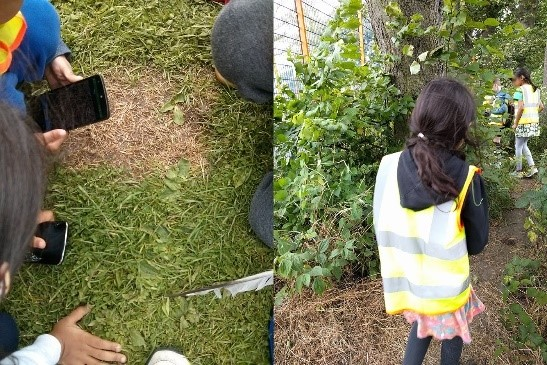
\includegraphics[width=0.8\columnwidth]{images/chapter04/prototypeDeployment.jpg}
  \caption[Children during the Park:Learn summer school deployment]{Groups of children finding and photographing habitats in a local park, using the Park:Learn prototype application.}
  \label{fig:prototypeDeployment}
\end{figure*}

We also wished to see how the prototype would be received by students, especially when used within the authentic learning environment of a park. Two deployments were held, with two groups of children in two different parks. In the first deployment (N=23, aged 4-12, recruited through an out of school club, in groups of 2-3 with a smartphone or tablet per group) students were given activities per their age: for younger children (age < 6. Figure 3, left), the app asked students to take photos of plants and wildlife, while older children (Figure 3, right) were additionally asked to Location Hunt items of historical significance in the park, record a short nature documentary style video and draw their vision of the park’s future on top of one of their own photographs (which some groups didn’t complete due to time limitations). These activities were inspired by worksheets that had previously been created by the park rangers and the discussions held with them. 

The second deployment was much more free-form in its activity design, taking place during a school group’s (N=55, aged 4-5, accessed through partnership with the schoolteacher) weekly visit to their local park. To fit into the teacher’s experiential, child-led approach for the visit, we wanted to present the application as an optional tool which children could engage with if they wished. To this end, we offered tablets running the application to 5 students (one device per child) who weren't engaging in other activities, such as tree climbing or playing in mud. The app was loaded with free-form activities which were designed to fit the child-led learning approach, encouraging the children to catalogue their findings during their usual self-guided explorations of the allocated park area in pictures and video. Of the 5 children we approached, 3 completed the app’s activities, while 2 disengaged when they realised that it wasn't a video-game.
Following these deployments follow-up interviews were held with the class teachers, with the aim to get feedback on the prototype and ideas for future developments.

\section{Engagement Insights}
\label{sec:InfrastructureInsights}
We found that the discussions which took place across these engagements highlighted three common elements: children's independent, self-guided learning; the role of place-making within citizenship; and the various tensions held by and between the park stakeholders.

\subsection{Self-Guided Civic Learning}

Discussions with the park rangers and teachers during the workshops and interviews revealed that, in their view, outdoor learning played a critical role in children’s development as citizens. They argued that the exposure of children to new experiences, environments and community members is an essential element which helps children to discover their passions and equip them to make decisions about their future. The concept of children exploring their environments to discover and nurture new interests through independent learning is a process which was raised repeatedly during our workshop discussions:

\begin{displayquote}
"They pick [these professions] because they are exposed to a wider variety of natural things, they have a choice to make. […] We shouldn’t just tie our pupils into traditional classroom activities. […] Expose children so that when they grow, they can become specialists." – Teacher 6
\end{displayquote}

Our workshop participants strongly believed that this process was reliant on children’s independence—if children were to find new interests and passions to take into later life, there would have to be significant degree of autonomy and freedom of learning. 

\begin{displayquote}
"It's about listening to the child and following what they want to do, as opposed to being subscribed.” – Ranger 2
\end{displayquote}

While this element of self-determination was recognised as important, it was also noted that the children would still often need a teacher’s presence to act as a facilitator and an enabler for the children’s explorative curiosity:

\begin{displayquote}
"It is much more about allowing the children to make their choices. […] You don’t do anything apart from facilitating and listening to them.” – Teacher 4
\end{displayquote}

Our participant teachers claimed that the children were discovering their passions over time through outdoor exploration, play and experimentation. Eventually, these would organically emerge into themes of personal interest which could be identified by their teachers.

\begin{displayquote}
"It’s about dealing with children’s own interests and passions. […] Maybe by February there’s some children who have a theme going.” – Teacher 7
\end{displayquote}

\begin{figure*}
  \centering
  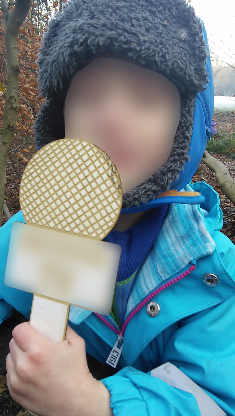
\includegraphics[width=0.4\columnwidth]{images/chapter04/microphone.png}
  \caption[A child completing a `Take a Video' Task]{A child documents his discoveries to the app during the second prototype deployment, using the `Take a Video' task and a cardboard microphone.}
  \label{fig:prototypeMicrophone}
\end{figure*}

We found that our initial design ideas (as with many existing mobile learning applications) were not particularly well suited to this process. Rather than allow for self-guided exploration and fluidity, our technology’s initial activity design in the first deployment had been prescriptive—meaning that the children were exploring our ideas, rather than their own. One of the more visible examples of this we saw was an activity which tasked young children to Photo Match images of types of leaves in the park. The children took this more literally than we expected, and tried to line the shot up perfectly with the leaf overlay. The result was the children cared more about taking the photograph than learning about the surrounding nature. The second deployment’s more open structure allowed for the application to take an embedded role in the session’s explorative activities—the technology became one of a selection of optional resources, including the park itself. For the participants who chose to utilise the technology, we saw that the creative potential of the application encouraged them to further engage in personal explorations of the park environment and document their discoveries (Figure \ref{fig:prototypeMicrophone}).

\subsection{Citizenship Through Place-making}

The teachers noted that as the children advanced through the early years of school, the focus of school activities changed from the sensory and experiential to the practical and applied. Project-based learning activities are introduced, allowing multiple school subjects to be taught around the periphery of a single class venture. In the school, an example of this was the development of the school’s garden and pond area. However, the rangers saw these projects as being opportunities for learning topics which extend beyond the current school curriculum.  They saw opportunities for civic learning, giving children an appreciation for the local parks and the work that goes into maintaining them. They wanted children to be able to explore the environment at their own pace, taking time to understand and appreciate it. Beyond this base appreciation, they hoped to instil a sense of ownership, belonging and responsibility. They wanted these learning activities to be place-making:

\begin{displayquote}
"Being involved in developing [the park], studying it. So that they feel like it's their park---not just some open space to throw cans in. […] They have ownership of it, the whole thing, and then maybe they’ll appreciate it and look after it." – Ranger 1
\end{displayquote}

For the rangers, working alongside the schools allowed them to teach children the civic value of parks. To them and the surrounding communities, the parks are more than just their physical components of open spaces, woodland and shrubbery. They have a true social value, something which needs to be treasured, nurtured and---crucially---communicated and passed-down. The rangers were very aware that the parks would soon be likely to be even more reliant on community support and volunteering. A possible route to future sustainability lies in instilling this sense of civic responsibility and duty of care. The activities designed to nurture this ownership tended to be creative in nature, allowing the children to feel like they had personally contributed to the spaces. Examples of the activities the rangers organised with schools included children creating artistic roundels to surround a new pond and designing and building a nature area. The aim was to use this newly produced area to build long lasting relationships between students and the space over the course of their academic careers: using it for experiential activities, creation and, eventually, study. 

\begin{displayquote}
"They're actually involved in making the park: they planted that willow, and they planted some bulbs. So, they've been involved while quite young in creating this wildlife area and taking ownership of it. Hopefully, once it's established, we can involve older kids in actually studying it." – Ranger 1
\end{displayquote}

The rangers hoped that these studies would again be mutually beneficial for both the schools and parks: as well as allowing the students opportunities for situated outdoor learning, the parks could benefit from the collected data. The students’ findings could be fed into organisations such as the Wildlife Trust and local citizen science projects, further increasing the perceived value of the parks to their surrounding communities.

There was a broad range of attitudes amongst our workshop participants concerning technology’s role in parks’ place-making. Some were critical, viewing many technologies as distractions from the learner’s environment: the rangers and teachers alike were concerned that if a child is focusing on the technology in their hands rather than what’s surrounding them, how can they form a meaningful relationship with that space? However, there was also optimism about the use of technology as a powerful tool within this space. Some saw it as a way of furthering students’ engagement with and appreciation of the natural environment:

\begin{displayquote}
"I think [recording] audio would be really interesting to just listen to what the park sounds like, […] because I don't think we listen to nature enough. […] Just appreciating it." – Teacher 2
\end{displayquote}

Other ideas included using technology as a tool through which the rich social history of the parks could be uncovered and contextualised. Through the app’s photo-matching activity, the rangers suggested that children could compare the park of today to that of a hundred years ago. These differences could be used to contextualise the changing attitudes towards the parks’ usage and upkeep, as well as foster an appreciation for the efforts of the parks’ current volunteers (a resource which wasn't previously required, due to the large number of paid staff).

\subsection{Stakeholder Tensions}

Despite Ofsted urging schools to perform more outdoor learning activities, many teachers struggle to take their lessons outside—especially into parks. Through the workshops and interviews, we found that many aspects of the economic and institutional infrastructures surrounding the parks and schools restricted the amount of outdoor learning that could be supported, making for a difficult design space.

Recurrent and obvious was the topic of funding, for both the schools and parks alike. Most parks have had their budgets cut to the extent that they now have fewer staff: where there may have once been dedicated educational officers, rangers are having to cover in their stead in addition to their previous duties. Thus, schools are now charged for educational activities to (partially) compensate for rangers’ time, which is always in high demand. Schools suffering from budget cuts also compound this, resulting in many choosing to stop utilising the rangers as resources for expert knowledge or even ceasing trips to parks altogether.

The nature of our society has also resulted in an unequal access to nature in many people’s lives. Indeed, many of the original Victorian parks were originally created for the health benefits of factory workers. For urban areas living with child poverty, parks are a valuable resource—both for access to nature and new social opportunities for civic learning. The theme of natural environments being social equalisers was present in our discussions: parks allow for children to exist, play and learn on a level playing field when extraneous factors are stripped away. The teacher of the class which partook in the second deployment noted in the interview afterwards:

\begin{displayquote}
"In the classroom, he's lost. He doesn't have a TV at home, his parents are very highly educated and he finds it hard to mix in with the other children. But in the woods, it's a level playing field, because there's no TV, there's no toys that match anything that they might have seen on a film or anything like that. I suppose, for him, it’s his day that he’s on a par with everybody else." – Teacher 7
\end{displayquote}

Through the discussions with workshop teachers, additional tensions were revealed.  One was the existence of a prejudice and stigma against learning outside of the classroom:

\begin{displayquote}
"One [parent] complained, and said they weren't in the learning environment. It was just this weird perception. The parents looked at it and saw `Look at those students relaxing, that’s not going to be a learning environment.'" – Teacher 5
\end{displayquote}

Despite the teacher claiming to have `never had as much focus as when they were just relaxed, lying in the grass', he found himself having to defend the practice against outside scepticism. Amongst other institutional requirements, this necessitates that teachers create schemes of work and collect evidence of learning. This target and evidence-based methodology clearly conflicts with the experiential, holistic approach used for children’s self-development. These highly structured, prescriptive formats result in little room for exploration and the unexpected. Furthermore, the targets set by the UK’s National Curriculum mean that schools must teach very specific topics and meet specific targets, limiting teachers’ creative control and freedom in their activity design. One ranger (who happened to be a retired teacher) claimed that toeing the line of the national curriculum has resulted in many teachers losing the ability to teach topics in a manner tailored to students’ interests:

\begin{displayquote}
“You couldn't do that now, because of the curriculum. It’s so structured. Many of the teachers have gone through that system now, and it’s hard for them to go back and think creatively about how do it---it’s been knocked out of them.” – Ranger 1
\end{displayquote}

The increasingly lofty and specific learning targets for slightly older children are also affecting what is being taught in the earlier years of their education. Many schools are aiming to get children up to target earlier in their school careers---forfeiting the holistic experiences for the rote-style learning found in the later stages of school. Resistance to these top-down influences appears to be on a per-school basis, with Teacher 7 explaining why her school still delivers the holistic sessions:

\begin{displayquote}
“The curriculum is so heavy now with the grammar: our Year 6s need to know what `fronted adverbials' are. […] That's so high now it’s just filtering down. The pressure on what the children need to be able to do is just increasing. And it's our way of saying `we value children’s imaginations and children being children', so we keep doing this.” – Teacher 7 
\end{displayquote}

However, the current institutional climate realistically only allows for these entirely free-form activities to take place during the earliest years of a child’s school life. For schools to be able to sustainably hold outdoor learning activities for older children within the existing school infrastructure, they must conform to the expectations of targets and evidence set upon them.

\section{The Social Design Space for Mobile Learning Technologies}

These engagements have shown us that civic mobile learning in parks---and more broadly in civic spaces---is a rich but challenging design context. It's clear that for a technology to be successful within these community spaces, it must be designed in consideration of the existing social ecosystems. This requires an awareness of the motivations of each place’s stakeholders and the relationships that exist between them. In our park context, a design must allow for teachers to work within a set of pre-determined parameters, with the resulting deliverables supplying evidence of learning. Similarly, rangers’ time and resources are precious due to their plethora of commitments and lack of funding, so the activity design and creation processes must be quick and easy to distribute. While teachers may aim to teach to a strict, pre-written curriculum, rangers might prefer to strengthen learners’ relationships with the park and instil a sense of ownership. The local government want the parks to remain valuable community resources, but don’t have the funding to allow the previous amount of spending to be sustainable. Technology can offer new opportunities to surface these complexities for use as civic learning resources.

\begin{figure*}
  \centering
  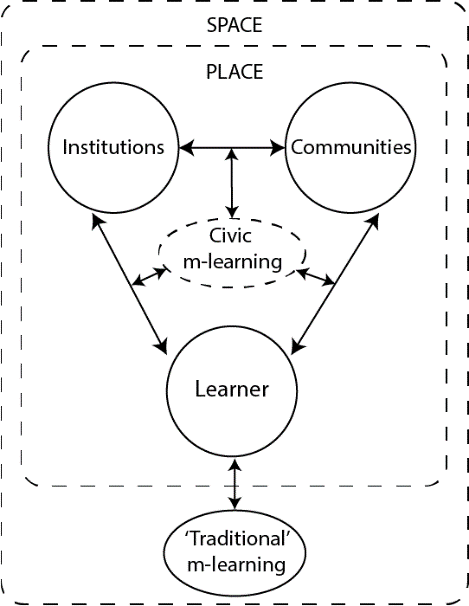
\includegraphics[width=0.45\columnwidth]{images/chapter04/designSpace.png}
  \caption[The social design space for mobile learning technologies]{The social design space for mobile learning technologies, where relationship infrastructures connect stakeholders in space and place. `Traditional' m-learning refers to mobile learning technologies which don’t meaningfully engage with these infrastructures, and are either independent of the learner’s context or concentrate solely on the physical aspects of the environment.}
  \label{fig:designSpace}
\end{figure*}

Based on our findings, we present a generalizable model of the social design space (Figure 1). In the model, we show how space and place (be they parks or schools) comprise of multiple actors: learners, communities, institutions and technologies. `Actors' refers to individuals who use the park as a space—be that learners, teachers, rangers, volunteers or other members of the public. `Communities' are multiple actors, united by a common interest, goal or issue: for example, ‘Friends of X Park’ volunteer groups, local residents and school groups. `Institutions' are those that impose requirements and/or restrictions on the other groups: for example, Ofsted or the city council. Each of these actors interact with the others through layers of infrastructure: for example, actors may exist within a community of practice and the city council may introduce financial tensions with the park rangers through policy. These infrastructures all contribute to comprising the park as a place.

However, most current mobile learning technologies only interact with the learners in physical space, oblivious of the socio-cultural, political and economic relationships that constitute place. If a technology is to be well suited for civic learning within this space, it needs to be produced with the interactions between stakeholders in mind. Civic mobile learning involves more than just the learner and the space in which they reside: it also involves other stakeholders' relationships---both with the space, and each other.

\section{Suggestions for Designing Technologies for Civic Learning}
\label{sec:SuggestionsCivicLearning}

This section presents some suggestions for designing technologies to support civic learning and extending the focus of m-learning technologies to include the social context, based on these findings and the identified design space.

\subsection{Create Opportunities for Giving Form to Stakeholder Values}

As suggested by Dourish and Bell, by considering the infrastructures that constitute a place/place, we can more easily understand the values that its surrounding communities associate with it \citep{Dourish2007}. Analysis of the different actors and stakeholders at play in a space offers researchers not only a greater appreciation of the multiple practices and values of it, but also opportunities to design technologies that accommodate them and bring them in relation to one another.

An awareness of the variety and import of stakeholder viewpoints, practices and values becomes even more necessary when the communication of these values is the technology’s defined purpose. In this project, the rangers' and teachers' agendas were very different, despite being stakeholders in the same space and place. Understanding the contexts and spatial infrastructures (socio-cultural, institutional, financial) where these values are enacted is key to designing appropriate technologies for civic learning in these spaces. We found that despite being major users of civic spaces such as parks (and therefore are stakeholders like any other actors), children’s values, practices and views regarding parks are often overlooked. Designing for civic mobile learning might entail the development of platforms that allows multiple stakeholders---including children---to express their values and practices and put them in dialogue with one another, encouraging political agency from an early age.

This potential can extend beyond the scope of individual places and communities operating within them. Indeed, m-learning technologies could operate as platforms for the sharing of values, practices and resources between and across different places and communities.  Bringing the practices and values in different communities and places into dialogue with one another can offer productive civic learning opportunities \citep{Wegerif2007}.  Fischer has also noted the need for collaboration amongst communities,  and claims that spatial, temporal, conceptual and technological barriers can be turned into creative opportunities \citep{Fischer2004}. Gryl and Jekel claim that the core competencies required for spatial citizenship are expression (constructing and communicating meanings of geographic information), communication (sharing those ideas and meanings with others) and negotiation (engaging in democratic discussion in an effort to find compatible meanings with others) \citep{Gryl2012}. Similarly, through activity creation, mobile learning applications like Park:Learn could be used to support learners’ active citizenship through surfacing other stakeholders’ values and practices and expressing the learner’s own. Future work could investigate how mobile learning technologies could assist in promoting engagement in further negotiation between stakeholders.

\subsection{Support Place-Making}

Through analysis of the workshops and interviews, it became clear that the process of independent learning and self-discovery was intrinsically linked to place-making. Children can explore and learn about their environment at will, allowing for unique and meaningful experiences to occur. The rangers were confident that these regular and meaningful interactions over time eventually lead to the formation of relationship between the learner and their environment. Yi-Fu Tuan claims that place-making is made possible through individuals ‘pausing’ in space to make it place \citep{Tuan1978}. However, we argue that rather than this passive act of pausing, place-making is promoted through doing---individuals entering an active engagement and creation process within a place and its infrastructures. To this end, outdoor learning technologies in this design space should support learners’ independent learning, curiosity and creativity. This was also seen in the second deployment of Park:Learn, where the creative potential offered by technology acted as a motivating factor.

The teachers noted that as the children progressed in age, they transitioned from experiential and explorative activities to creative ones in which they were actively affecting their environment (and effecting change). Civic learning technologies should support this transition into active participation within society. The rangers saw this as a means of place-making: by actively having a hand in the creation of areas of the park, children would be taking ownership and forming relationships with it. The rangers’ values where embedded into these activities, in the hope of them being passed onto a new generation. To assist in this process, mobile learning technologies might act as both creative tools and social infrastructure: empowering users to create new unique works, and share and absorb the knowledge of others in a place’s community through an ongoing dialogue and exchange between the learners and other stakeholders. As an example of how this could be implemented in a mobile learning application, communities could create their own activities in Park:Learn to form their own informal curricula: sharing values, knowledge and promoting place-making through situated learning.

\subsection{Balance the Use of Technology}
\label{sec:BalanceTechUse}

Through these extensive engagements, it appeared that stakeholders’ perceptions of the role technology might play in parks weren't always positive. Some of our participants saw the inclusion of technology as something that could distract from the learning experience and place-making. This is a criticism which could be levelled at projects such as \citep{Shih2010}, which shows a photograph of a class visiting a temple, engrossed in their mobile devices rather than the environment around them. As civic learning is tied to practices of place-making, when designing for civic mobile learning we must be mindful not to place technology at the `centre': a technology designed for civic education and place-making should not presume itself to be the learning objective, and instead take a background supporting role. We must acknowledge that there are situations where the very inclusion of technology may not be appropriate. For example, the inclusion of a technology could completely negate explorative outdoor learning’s equalising effects if not all children are familiar with it. As HCI designers, we must recognise and appreciate that the value of a physical or social space could be jeopardised by heavy-handed outside involvement—sometimes the lack of technology in a space could be why it is precious to begin with.

\begin{figure*}
  \centering
  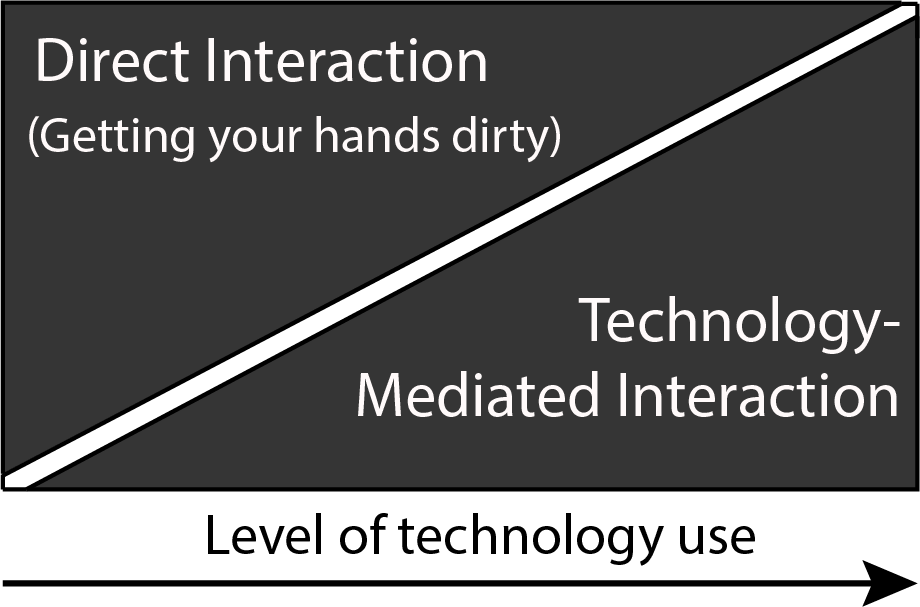
\includegraphics[width=0.45\columnwidth]{images/chapter04/techBalance.png}
  \caption[Balancing technology use]{Balance the amount of direct and technology-mediated interactions to find the 'sweet-spot' for civic learning.}
  \label{fig:techBalance}
\end{figure*}

However, technologies can offer new learning opportunities which might not otherwise be possible or feasible. For example, mobile learning can give stakeholders platforms to communicate their own values and motives concerning place; expose the values of others to learners across time and space; augment physical reality with digital information; and allow for dynamic and creative learning activities thanks to the available networking and hardware features. Thus, a careful balance must be maintained between the potential benefits of civic m-learning’s inclusion and the risk of its overuse. A `sweet spot' (specific to the learner and the learning context) can be found in the space between completely direct, hands-on activities without any technology use and a fully technology-mediated approach. As the focus on one increases, the other decreases, and their respective benefits follow (Figure \ref{fig:techBalance}). 

\section{Summary}

This chapter gave an overview of this PhD project's origins. Motivated by the visible impact of austerity politics on local parks---particularly the educational services which they had previously provided---I started investigating the resources that these spaces offered, their use by local schools, the relationships held with them by their surrounding communities, the constraints and tensions felt by the stakeholders which regularly engaged with them as places, and how mobile learning technologies could be used to surface these elements as learning material. These initial studies resulted in a greater understanding of the design space for engaging with a place's social infrastructures as learning resources, and how mobile technologies can be more suitably designed for civic learning.

Contextually, these studies engaged with the results of the austerity politics that originally inspired the Digital Civics agenda. It was clear that the funding cuts had drastically impacted the way that park rangers managed the spaces, with them becoming much more reliant on community volunteerism. While this seemed to be working in a few (typically affluent) areas, the rangers were afraid that it wasn't sustainable for the majority in the long-run. A reduction of full-time staff meant that educational activities were given significantly less support, meaning that existing educational resources and the expertise of the rangers themselves were going underutilised. In response, I proposed a design for the mobile application Park:Learn. This app could be used by schools and communities to make use of the rangers' knowledge, without requiring their immediate presence.

This application was prototyped, and used as a technology probe during engagements with stakeholders (teachers, students, park rangers and volunteers) to which the participants were receptive. These engagements were useful in promoting discussion around the importance of students' self-guidance, the promotion of active citizenship through building relationships with community spaces, and the various tensions held by the stakeholders in their relationships to the parks as places. Using these insights, we illustrated a design space which highlights the different stakeholders’ current issues and practices. With minor adaptation, this model should be adaptable for civic mobile learning in settings other than parks. We also offered some implications for designing platforms that support outdoor civic learning activities and place-making, highlighting the importance of creating opportunities for stakeholders to give form to and share their values with others; encourage place-making by supporting independent learning, curiosity and creativity; and the need for an awareness of the over-use of technology to be a disruptive and negative factor when learning in authentic environments.

